17. \begin{figure}[ht!]
\center{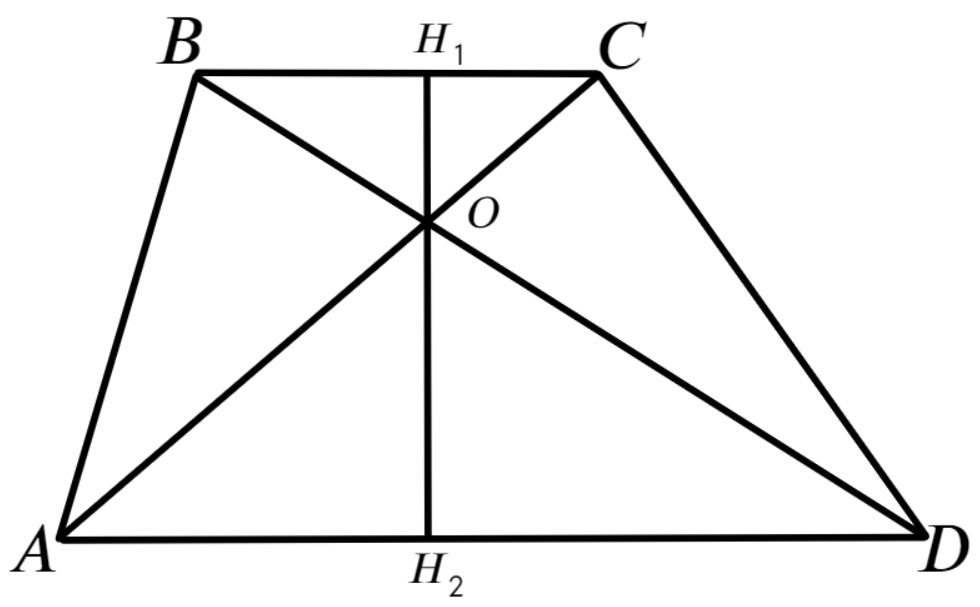
\includegraphics[scale=0.35]{g9-17.png}}
\end{figure}\\
Треугольники $BOC$ и $AOD$ подобны по двум углам (накрест лежащим $OBC$ с $ADO$ и $OAD$ с $OCB$), коэффициент подобия $k=\sqrt{\cfrac{S_{\Delta BOC}}{S_{\Delta AOD}}}=\sqrt{\cfrac{a^2}{b^2}}=\cfrac{a}{b}.$ Пусть тогда $BC=ax,\ AD=bx.$ Высоты в подобных треугольника относятся друг к другу с тем же коэффициентом подобия, поэтому можно считать, что $OH_1=ay,\ OH_2=by.$ При этом $S_{\Delta BOC}=\cfrac{1}{2}\cdot ay\cdot ax=a^2,$ откуда $xy=2.$ Таким образом, $S_{ABCD}=\cfrac{BC+AD}{2}\cdot H_1H_2=\cfrac{ax+bx}{2}\cdot(ay+by)=(a+b)^2.$\\
